\documentclass[11pt]{article}

\usepackage{url}
\usepackage{enumerate}
\usepackage{pifont}
\usepackage{longtable}
\usepackage[hidelinks]{hyperref}
\usepackage{graphicx}
\usepackage{caption}
\usepackage{subcaption}
\usepackage{tikz}
\usetikzlibrary{arrows,shapes}
\usepackage{pifont}

\begin{document}

\title{\textbf{Axe Manual}\\ {\large Version 1.2, March 2016}}
\author{Matthew Naylor and Simon Moore, \\
University of Cambridge Computer Laboratory}
\date{}
\maketitle

\tableofcontents

\newpage

\setlength{\parskip}{1em}
\renewcommand{\thefootnote}{\fnsymbol{footnote}}

\newcommand{\cmark}{\ding{51}}
\newcommand{\xmark}{\ding{55}}

\section{Introduction}

Axe is a tool that aids automatic, black-box testing of the
memory subsystems found in modern multi-core processors.  Given a
trace containing a set of top-level memory requests and responses, Axe
determines if the trace is valid according to a range of \emph{memory
consistency models}.  It is designed to be used as the oracle in an
automated hardware test framework, quickly checking large memory
traces that result from randomly-generated sequences of memory
operations \cite{BlueCheck}.
It can also assist bug diagnosis by enabling
testing strategies that search
for small failing cases \cite{BlueCheck}.
Despite
the large amount of non-determinism present in memory consistency
models, Axe can handle long traces involving many cores.

Axe supports a spectrum of five consistency models listed in Table
\ref{Table:Models}, each one permitting a subset of the behaviours
allowed by the next and supporting a greater number of implementation
features.

We validate Axe by various means: (1) by testing it for equivalence
against existing models developed by others; (2) by testing
equivalence between optimised and non-optimised versions of the same
model; and (3) by applying it to traces generated by real and model
hardware implementations.

\begin{table}
\renewcommand{\arraystretch}{1.5}
\begin{center}
\begin{tabular}{llll}
          & \textbf{Model}  & \textbf{Expansion} & \textbf{Supports feature} \\
          & SC     & Sequential Consistency \cite{SC} \\
$\subset$ & TSO    & Total Store Order \cite{SPARC} & Store buffering \\
$\subset$ & PSO    & Partial Store Order \cite{SPARC} & Out-of-order writeback \\
$\subset$ & WMO\footnotemark[2]
                   & Weak Memory Order \cite{SPARC} & Load buffering and \\
          &        & & out-of-order responses \\
$\subset$ & POW    & POWER model \cite{POWER} & Multiple shared caches \\
          &        & & and lazy invalidation
\end{tabular}
\end{center}
\caption{Total order of supported memory consistency models.}
\label{Table:Models}
\end{table}

\footnotetext[2]{WMO is equivalent to SPARC RMO \cite{SPARC} except
that it forbids reordering of loads to the same address, making it a
subset of modern relaxed models such as POWER \cite{POWER}.}

Axe is available from \url{http://www.github.com/CTSRD-CHERI/axe}.
(The name ``Axe'' comes from the use of axiomatic rules to decide the
validity of traces.)

\subsection{Problem definition}
\label{Section:ProbDef}

Given a trace containing a set of memory requests and responses
(including loads, stores, atomic read-modify-writes, memory barriers,
and optional timestamps) initiated by concurrent processor cores (or
``hardware threads''), Axe determines if the trace satisfies one of
the consistency models listed in Table \ref{Table:Models}.  We define
the memory trace format in \S\ref{Section:TraceFormat} and give an
operational semantics for each of the consistency models in
\S\ref{Section:SPARCModels} and \S\ref{Section:POWERModel}.

Following Gibbons \cite{Gibbons} and Manovit\cite{Manovit}, we assume
that the address-value pair of every store in a trace is unique, i.e.
the same value is never written to the same address twice.  This
reduces the amount of non-determinism in a model as it allows the
store read by any load to be uniquely identified. This restriction is
easily met by an automatic test generator and is justified by the
fact that the actual values being stored do not typically affect any
interesting hardware behaviour.  But it does mean that our tool cannot
be used for checking memory traces that arise during execution of
arbitrary software applications, which are unlikely to meet this
restriction.

Another technique for reducing non-determinism is to modify the
hardware to emit extra trace information such as the order in which
writes reach a particular internal merge point.  However, for now we
treat the memory subsystem as a \emph{black box} and do not inspect or
modify its internals in any way.  The reason for this is that we would
like our tool to be as easy as possible to use, i.e. not requiring
modifications to the system under test.


\subsection{Background}

Axe is part of our efforts to support testing and debugging of the
CHERI processor developed at the University of Cambridge and SRI
International \cite{CHERI}.  It is heavily inspired by Manovit's
\emph{TSOTool} \cite{Manovit,TSOTool} which randomly generates SPARC
programs, runs them, and checks the resulting traces for consistency.
This is exactly the kind of approach we had envisaged for testing our
own memory subsystem, except for the generation of ISA-level programs
rather than direct HDL-level memory requests.  The performance of
TSOTool is impressive, scaling to large traces involving many cores.
Unfortunately, ``TSOTool is a proprietary program of Sun Microsystems''
\cite{TSOTool}, and only supports the TSO model.  Our checking
algorithm for the SC, TSO, PSO and WMO models is a mild generalisation
of Manovit's algorithm, and has a freely-available implementation.

Our work is also influenced by the memory model by Sarkar et al.
\cite{POWER} for the IBM POWER architecture, and the associated
simulator, PPCMEM \cite{PPCMEM}.  Although PPCMEM is not designed for
efficient trace-checking and can take a very long time to terminate
even on very small traces (of less than ten instructions on a few
threads), this work has greatly helped our understanding of modern
relaxed memory models as well as assisting our testing of Axe.

\section{Trace format}
\label{Section:TraceFormat}

We introduce the syntax of memory-subsystem traces by way of example.

\paragraph{Example 1} Here is a simple trace consisting of five
operations running on two threads.  

\begin{verbatim}
0: M[1] := 1
0: sync
0: M[0] == 0
1: M[0] := 1
1: M[1] == 0
\end{verbatim}

\noindent The number before the \verb#:# denotes the thread id.  The
first line can be read as: thread \verb#0# stores value \verb#1# to
memory location \verb#1#.  The second line as: thread \verb#0#
performs a memory barrier.  And the final line as: thread \verb#1#
reads value \verb#0# from memory location \verb#1#.

The initial value of every memory location is implicitly \verb#0#.
For any read of a value other than \verb#0#, there must exist a write
of that value to the same address in the trace, otherwise the trace is
said to be malformed.  As mentioned in \S\ref{Section:ProbDef}, we
also require that the address-value pair of every write is unique.

The textual order of operations with the same thread id is the order
in which those operations were submitted to the memory subsystem by
that thread.  Following standard terminology, we refer to this order
as \emph{program-order}.  No ordering is implied by the textual order
of operations with different thread ids.  In the above example, the
write by thread \verb#1# is not ordered in any way with respect to any
of the operations by thread \verb#0#, but it is program-order-before
the read by thread \verb#1#.

\paragraph{Example 2} Here is another trace, illustrating timestamps.

\begin{verbatim}
0: M[0] := 1
0: sync
0: M[1] := 1
1: M[1] == 1    @ 100 : 110
1: M[0] == 0    @ 115 :
\end{verbatim}

\noindent The operation on the fourth line contains a begin-time of
\verb#100# and an end-time of \verb#110#, denoting the times at which
the request was submitted and the response received respectively.
Operations that perhaps do not generate a response, such as a store,
can simply leave the end-time unspecified\footnote{Axe
currently disallows end-times for store operations, making it clear
that this information is not used.}.  In fact,
all timestamps are completely optional, for two reasons:

\begin{itemize}

\item some consistency models are unaffected by timestamp information;

\item example traces are easier to read if only the interesting or
relevant timestamp information is supplied.

\end{itemize}

In some consistency models however, timestamps do affect whether or
not a trace is allowed.  In the above example, the timestamps indicate
that first load by thread \verb#1# must have finished before the
second load by thread \verb#1# begins which might imply that the
memory subsystem could not have executed the operations out-of-order.
In the SPARC and POWER architectures, a programmer can arrange such a
dependency by having the address of the second load be dependent on
the result of the first load -- a so-called \emph{address dependency}
[7].  Other kinds of dependency include \emph{data dependencies} (where
the value of a store is dependent on the result of a preceding load)
and \emph{control dependencies} (where an operation is control-flow
dependent on the result of preceding load).  All these program-level
dependencies become observable in the memory trace as
end-time-before-begin-time dependencies.

By default, we consider timestamps to be \emph{local to each thread},
i.e. we do not use timestamps to infer ordering between operations
that run on different threads.  This means we can test hardware in
which the threads are running in separate clock domains, for example.
However, if the \verb!-g! command line flag is specified then Axe can
assume a global clock, and compare timestamps of operations running on
different threads.  Currently, we only exploit the \verb!-g! flag in
our POW model\footnote{Specifically, we infer an ordering between two
\texttt{sync} operations running on different threads if the one ends
before the other begins.}.

\paragraph{Example 3} Here is third trace, this time containing
three operations, the first of which is an atomic read-modify-write
operations.

\begin{verbatim}
0: <M[0] == 0; M[0] := 1>
1: M[0] := 2
1: M[0] == 1
\end{verbatim}

\noindent The first line can be read as: thread \verb#0#
\emph{atomically} reads value \verb#0# from memory location \verb#0#
and updates it to value \verb#1#.  The two memory addresses in an
atomic operation must be the same, otherwise the trace is malformed.
A common way of expressing atomic operations in RISC instruction sets
is via a pair of \emph{load-linked} and \emph{store-conditional}
operations.  At the trace level, it is straightforward to convert such
a pair of operations into a single read-modify-write operation:

\begin{itemize}

\item if the store-conditional fails, then remove it from the trace
and convert the load-linked to a standard load;

\item otherwise, convert both operations to a single read-modify-write
operation.

\end{itemize}

\noindent For read-modify-write operations, the end-time simply
denotes the time at which the read-response is received.  Currently,
Axe has no concept of an end-time on a write operation.

\paragraph{Example 4} The following trace illustrates \verb#final#
constraints.

\begin{verbatim}
0: M[0] := 1
0: M[1] := 1
1: M[1] := 2
1: M[0] == 0
final M[1] == 2
\end{verbatim}

\noindent The \verb#final# line states that final value at location
\verb#1# viewed by all threads after all operations have completed
is \verb#2#.  These \verb#final# constraints are entirely optional and
are primarily supported so that litmus tests (used for testing our
models) can be neatly expressed as traces.

\section{Command-line usage}
\label{Section:CmdLine}

Axe can be invoked as follows:
\begin{verbatim}
  axe check <MODEL> <FILE> [-g]
\end{verbatim}
\noindent where \verb!<MODEL>! is \verb!SC!, \verb!TSO!, \verb!PSO!,
\verb!WMO!, or \verb!POW!; \verb!<FILE>! is the name of file
containing a trace (\S\ref{Section:TraceFormat}) or ``\verb!-!'' to read a
trace from standard input.  The optional \verb!-g! flag (currently
only used in the \verb!POW! model) indicates that a global clock domain
may be assumed (see \S\ref{Section:TraceFormat} for more details).

The output is either ``\verb!OK!'', denoting that the trace is allowed by
the specified model, or ``\verb!NO!'' if it is forbidden.  If the trace is
malformed or does not meet the necessary constraints, an error message
will be reported.
To illustrate, if the file \verb!trace.axe! contains:
\begin{verbatim}
  0: M[1] := 1
  0: M[0] == 0
  1: M[0] := 1
  1: M[1] == 0
\end{verbatim}
\noindent then the command
\begin{verbatim}
  axe check TSO trace.axe
\end{verbatim}
\noindent will output ``\verb!OK!''.

\subsection*{Multiple traces per file}

Axe allows a single file to contain multiple traces, with each trace
terminated by a line containing the text ``\verb!check!''.  It also allow
comments (lines beginning with the character ``\verb!#!'') in trace
files.
To illustrate, if the file \verb!traces.axe! contains:
\begin{verbatim}
  # Trace 1
  0: M[1] := 1
  0: M[0] == 0
  1: M[0] := 1
  1: M[1] == 0
  check

  # Trace 2
  0: M[0] := 1
  0: M[1] := 1
  1: M[1] == 1
  1: M[0] == 0
  check
\end{verbatim}
\noindent then the command
\begin{verbatim}
  axe check TSO traces.txt
\end{verbatim}
\noindent will output:
\begin{verbatim}
  OK
  NO
\end{verbatim}
\noindent That is, one decision per trace, in order.

\subsection*{Interaction}

It is straightforward to connect Axe to other tools such as HDL
simulators: any program can simply \verb!popen()! Axe, specifying the
input file as ``\verb!-!'', and communicate with it via pipes.

\subsection*{Testing}

Axe also supports the invocation pattern:
\begin{verbatim}
  axe test <MODEL> <FILE> <FILE> [-g]
\end{verbatim}
\noindent where the arguments are the same as before, except for the
introduction of the
second \verb!<FILE>! argument which specifies a file of expected
outcomes (i.e. ``\verb!OK!'' or ``\verb!NO!''), one for each trace in the trace
file.  Axe reports an error if any trace does not give
the expected outcome.  The purpose of this mode is to support testing of
Axe itself.  There are a large number of tests and expected outcomes
in the ``\verb!tests!'' subdirectory of the Axe distribution.

\subsection*{Shrinking traces}

When a trace fails a given consistency model, Axe
simply reports back ``\verb!NO!''.  This is not particularly helpful
in understanding \emph{why} a trace is invalid,
especially when
long.  In such cases, the \verb!axe-srhink.py! script
(included in the \verb!src! subdirectory) can be used to find the
smallest subset of the trace that fails the model.
To illustrate, suppose the file \verb!failure.axe! contains a 260-line
trace that fails the TSO model.  Running
\begin{verbatim}
  axe-shrink.py TSO failure.axe
\end{verbatim}
might give:
\begin{verbatim}
  Pass 0
  Omitted 241 of 260         
  Pass 1
  Omitted 256 of 260         
  Pass 2
  Omitted 256 of 260         
  0: M[2] := 46 @ 497:
  1: M[2] == 46 @ 280:513
  1: M[2] := 61 @ 729:
  1: M[2] == 46 @ 854:979
\end{verbatim}

\noindent The 260-line trace has been reduced to 4 lines.  This simple
trace shrinker, included in the Axe distribution, is often effective
but also rather slow for very large traces.

\section{SPARC models}
\label{Section:SPARCModels}

This section presents an operational semantics for the SC, TSO, PSO
and WMO models supported by Axe.  We define the behaviours allowed by
each model using an abstract machine consisting of a state and a set
of state-transition rules.  In each case, the state consists of:

\begin{itemize}

\item A trace $T$ (a sequence of operations in the format given in
\S\ref{Section:TraceFormat}).

\item A mapping $M$ from memory addresses to values.

\item A mapping $B$ from thread ids to sequences of operations.  We
call $B(t)$ the \emph{local buffer} of thread $t$.

\end{itemize}

In the \emph{initial state}, $T$ is the trace we wish to check, $M(a)
= 0$ for each address $a$, and $B(t) = []$ for each thread $t$.
(Notation: $[]$ denotes the empty sequence.)

Using the state-transition rules, if there is a path from the initial
state to a state in which $T = []$ and $B(t) = []$ for all threads
$t$, where $M$ satisfies all the \verb#final# constraints in this
final state, then we say that the machine accepts the initial trace
and that the trace $T$ is allowed by the model.  Otherwise, it is
disallowed by the model.

\subsection{Sequential Consistency (SC)}

SC has just one state-transition rule.

\paragraph{Rule 1}

Pick a thread $t$ non-deterministically.  Remove the first operation
$i$ executed by $t$ from the trace.

\begin{enumerate}
\item
     If $i = \texttt{M[}a\texttt{]:=}~v$ then update $M(a)$ to $v$.

\item
     If $i = \texttt{M[}a\texttt{]==}~v$ and $M(a) \neq v$
     then $\textbf{fail}$.

\item
     If $i = \texttt{<M[}a\texttt{]==}~v_0\texttt{; M[}a\texttt{]:=}~v_1
     \texttt{>}$ then:

\begin{enumerate}[i]
\item
          if $M(a) \neq v_0$ then $\textbf{fail}$;
\item
          else: update $M(a)$ to $v_1$.
\end{enumerate}
\end{enumerate}

\noindent We use the term $\textbf{fail}$ to denote that the
transition rule \emph{cannot} be applied under the chosen values for
the non-deterministic variables.  In this case $t$ is the only
non-deterministic variable.  

\subsection{Total Store Order (TSO)}

In TSO, each thread has a local store buffer.  Before presenting the
semantics, we give a few examples of TSO behaviour.

\paragraph{Example (SB)} Here is a sample trace that is allowed by
TSO but forbidden by SC.

\begin{verbatim}
0: M[1] := 1
0: M[0] == 0
1: M[0] := 1
1: M[1] == 0
\end{verbatim}

\noindent There is no interleaving of the operations that results in both reads
returning zero.  However, under TSO, a write may be buffered locally
by a thread, allowing a subsequent load to complete before the write
can be seen by another thread.

\paragraph{Example (SB+syncs)}  Under TSO, the above behaviour can be
prevented by inserting \verb!sync! operations that cause the local
buffers to be flushed.  The following trace is forbidden.

\begin{verbatim}
0: M[1] := 1
0: sync
0: M[0] == 0
1: M[0] := 1
1: sync
1: M[1] == 0
\end{verbatim}

\noindent In general, placing a \verb!sync! between every pair of program-order
operations restores SC behaviour.

\paragraph{Example (SB+RMWs)} Another interesting way to prevent the
relaxed behaviour in the SB example is to replace each write with an
atomic read-modify-write.  The following trace is forbidden.

\begin{verbatim}
0: { M[1] == 0; M[1] := 1 }
0: M[0] == 0
1: { M[0] == 0; M[0] := 1 }
1: M[1] == 0
\end{verbatim}

\noindent The atomic operations require that update be made
globally, not on a local copy, and since TSO prevents reordering of
writes, an atomic operation will have the effect of flushing the write
buffer.

\subsubsection*{Operational Semantics}

We define TSO using two rules.  The first is similar to Rule 1 of SC,
modified to deal with writing to and reading from the store buffers.
The second deals with evicting elements from the buffers to memory.

\paragraph{Rule 1}

Pick a thread $t$ non-deterministically.  Remove the first operation
$i$ executed by $t$ from the trace.

\begin{enumerate}
\item 
     If $i = \texttt{M[}a\texttt{]:=}~v$ then append $i$ to $B(t)$.

\item 
     If $i = \texttt{M[}a\texttt{]==}~v$ then let $j$ be the latest
     operation of the form $\texttt{M[}a\texttt{]:=}~w$ in
     $B(t)$ and:
     
       i.   if $j$ exists and $v \neq w$ then $\textbf{fail}$.

       ii.  if $j$ does not exist and $M(a) \neq v$ then $\textbf{fail}$;

\item 
     If $i = \texttt{sync}$ and $B(t) \neq []$ then $\textbf{fail}$.

\item
     If $i = \texttt{<M[}a\texttt{]==}~v_0\texttt{; M[}a\texttt{]:=}~v_1
     \texttt{>}$ then:

\begin{enumerate}[i]
\item
           if $B(t) \neq []$ then $\textbf{fail}$;

\item
           else if $M(a) \neq v_0$ then $\textbf{fail}$;

\item
           else: update $M(a)$ to $v_1$.
\end{enumerate}
\end{enumerate}

\paragraph{Rule 2}

Pick a thread $t$ non-deterministically. Remove the first operation
$\texttt{M[}a\texttt{]:=}~v$ from $B(t)$ and update $M(a)$ to v.

\subsection{Partial Store Order (PSO)}

PSO is similar to TSO but relaxes the order in which writes can be
evicted from the buffer.  In particular: writes to different addresses
can be evicted out-of-order.

\paragraph{Example (MP)} The following trace is allowed by PSO but
forbidden by TSO.

\begin{verbatim}
0: M[0] := 1
0: M[1] := 1
1: M[1] == 1
1: M[0] == 0
\end{verbatim}

\noindent The writes may be evicted \emph{out-of-order} from the local
buffer on thread 0, allowing thread 1 to see the second write before
it sees the first.

\paragraph{Example (MP+sync+po)} The above relaxed behaviour can be
prevented by inserting a \verb!sync! between the writes.  The
following trace is forbidden by PSO.

\begin{verbatim}
0: M[0] := 1
0: sync
0: M[1] := 1
1: M[1] == 1
1: M[0] == 0
\end{verbatim}

\paragraph{Example (MP+RMWs)}  Under TSO, atomic operations have the
side-effect of flushing the local write buffer.  Under PSO, only
writes to the same address are flushed, hence the following trace
is allowed under PSO.

\begin{verbatim}
0: M[0] := 1
0: { M[1] == 0; M[1] := 1 }
1: M[1] == 1
1: M[0] == 0
\end{verbatim}

\subsubsection*{Operational Semantics}

\paragraph{Rule 1}

This is identical to Rule 1 of TSO except that clause 4 becomes:

\begin{enumerate}
\setcounter{enumi}{3}
\item
     If $i = \texttt{<M[}a\texttt{]==}~v_0\texttt{; M[}a\texttt{]:=}~v_1
     \texttt{>}$ then:
\begin{enumerate}[i]

\item
           if any operation in $B(t)$ refers to address $a$ then
           $\textbf{fail}$;

\item
           else if $M(a) \neq v_0$ then $\textbf{fail}$;

\item
           else: update $M(a)$ to $v_1$.
\end{enumerate}
\end{enumerate}

\paragraph{Rule 2}

Non-deterministically pick a thread $t$ and an address $a$.  Remove
the first operation that refers to address $a$,
$\texttt{M[}a\texttt{]:=}~v$, from $B(t)$ and update $M(a)$ to $v$.

\subsection{Weak Memory Order (WMO)}

WMO is a relaxation of PSO in which load operations, like stores,
become non-blocking.  Unlike SPARC's RMO, it forbids reordering of
loads to the same address, making it a subset of modern relaxed models
such as POWER.  In all other respects, it is equivalent to RMO.

\paragraph{Example (MP+sync+po resisted)} This example, forbidden by
PSO, is allowed by WMO because the while the writes must occur in
order, the loads (to different addresses) may happen out-of-order.

\paragraph{Example (MP+syncs)}  If a sync is also placed between the
two loads as follows, then the relaxed behaviour becomes forbidden.

\begin{verbatim}
0: M[0] := 1
0: sync
0: M[1] := 1
1: M[1] == 1
1: sync
1: M[0] == 0
\end{verbatim}

\paragraph{Example (MP+sync+dep)} Alternatively, a dependency between
the two loads, in the form of a ``begin-time after an end-time'' may
also be used to keep the loads in order.  The following trace is
forbidden by WMO.

\begin{verbatim}
0: M[0] := 1
0: sync
0: M[1] := 1
1: M[1] == 1   @ 100:110
1: M[0] == 0   @ 115:
\end{verbatim}

\noindent The fact that the second load begins after the first one
completes is enough, under WMO, to imply that the memory subsystem
cannot reorder them.

\subsubsection*{Operational Semantics}

\paragraph{Rule 1} 

Pick a thread $t$ non-deterministically.  Remove the first operation
$i$ executed by $t$ from the trace.

\begin{enumerate}
\item
     If $i = \texttt{sync}$ and $B(t) = []$ then succeed;
\item
     Otherwise: $\textbf{fail}$.
\end{enumerate}

\paragraph{Rule 2}

Non-deterministically pick a thread $t$ and an address $a$.  From the
trace, remove the first operation $i$ on thread $t$ that satisfies the
condition: (a) $i = \texttt{sync}$; or (b) $i$ accesses address $a$
and no operation that precedes $i$ in program-order has an end-time
that precedes the begin-time of $i$.

\begin{enumerate}
\item 
     If $i = \texttt{sync}$ then $\textbf{fail}$.

\item 
     If $i = \texttt{M[}a\texttt{]:=}~v$ then append $i$ to $B(t)$.

\item 
     If $i = \texttt{M[}a\texttt{]==}~v$ then let $j$ be the latest
     operation of the form $\texttt{M[}a\texttt{]:=}~w$ in
     $B(t)$ and:
     
       i.   if $j$ exists and $v \neq w$ then $\textbf{fail}$.

       ii.  if $j$ does not exist and $M(a) \neq v$ then $\textbf{fail}$;

\item
     If $i = \texttt{<M[}a\texttt{]==}~v_0\texttt{; M[}a\texttt{]:=}~v_1
     \texttt{>}$ then:

\begin{enumerate}[i]
\item
           if $B(t) \neq []$ then $\textbf{fail}$;

\item
           else if $M(a) \neq v_0$ then $\textbf{fail}$;

\item
           else: update $M(a)$ to $v_1$.
\end{enumerate}
\end{enumerate}

\paragraph{Rule 3}

Non-deterministically pick a thread $t$ and an address $a$.  Remove
the first operation that refers to address $a$,
$\texttt{M[}a\texttt{]:=}~v$, from $B(t)$ and update $M(a)$ to $v$.

\subsection{Axiomatic definitions}

This section presents the axiomatic definitions of the SC, TSO, PSO and
WMO models upon which which the Axe checking algorithm for these
models is based.  In this section, we consider a read-modify-write
operation to be both a ``load'' and a ``store''.

To begin, it is helpful to distinguish between two different orderings
over operations in the trace:

\begin{itemize}

\item
\emph{Program Order}: for any given thread, the textual order of
operations in the trace issued by that thread.

\item
\emph{Memory Order}: a total order over all operations in the trace.

\end{itemize}

All valid traces under under these models must satisfy the following
property (\textbf{value axiom}): the value returned by a load from
address $a$ equals the value of the latest store (in memory
order) from the set $Local \cup Global$ where $Local$ is the set of
stores to address $a$ that precede the load in \emph{program order}
and $Global$ is the set of stores to address $a$ that precede the load
in \emph{memory order}.

Depending on the model, the following \textbf{local axioms} on
program-order operations $i$ and $j$ must also be satisfied.

\subsubsection*{Sequential Consistency (SC)}

If $i$ precedes $j$ in program-order then $i$ must precede
$j$ in memory order.

\subsubsection*{Total Store Order (TSO)}

If $i$ precedes $j$ in program-order then $i$ must precede
$j$ in memory order \textbf{when}:

\begin{itemize}
\item $i$ is a load; or
\item $i$ and $j$ are stores; or
\item $i$ is a \verb!sync! or $j$ is a \verb!sync!.
\end{itemize}

\subsubsection*{Partial Store Order (PSO)}

If $i$ precedes $j$ in program-order then $i$ must precede
$j$ in memory order \textbf{when}:

\begin{itemize}
\item $i$ is a load; or
\item $i$ and $j$ are stores \emph{to the same address}; or
\item $i$ is a \verb!sync! or $j$ is a \verb!sync!.
\end{itemize}

\subsubsection*{Weak Memory Order (WMO)}

If $i$ precedes $j$ in program-order then $i$ must precede
$j$ in memory order \textbf{when}:

\begin{itemize}

\item $i$ is a load and $j$ accesses the same address; or

\item $i$ and $j$ are stores to the same address; or

\item $i$ is a \verb!sync! or $j$ is a \verb!sync!; or

\item $i$ is a load with end-time $t_0$ and $j$ has begin-time
$t_1$ and $t_0 < t_1$.

\end{itemize}

\subsection{Checking algorithm}

In this section, we generalise an algorithm by Manovit \cite{Manovit}
for checking traces against the TSO model to support the SC, TSO, PSO
\emph{and} WMO models.  The central data structure used by this
algorithm is the \emph{analysis graph} in which each node denotes an
operation from the trace, and each edge denotes that the source node
precedes the destination node in memory order.

%Note that the analysis graph represents a partial order.

\subsubsection*{Simple algorithm}

Starting with an empty analysis graph, a simple checking algorithm is
as follows.

\begin{enumerate}

\item Add each operation in the trace as a node to the analysis graph.

\item Add the edges implied by the local axioms defined
above.

\item Apply the two edge-introduction rules shown in Figure
\ref{Fig:IntroRules} to the graph. 

\item Add an edge from each read $\texttt{M[}x\texttt{] == 0}$ to the
first program-order store $\texttt{M[}x\texttt{] := }a$ on each
thread.  This ensures that any read of zero (initial value) from
address $x$ must happen before any writes to address $x$.

\item Apply a standard topological sort procedure to the analysis
graph with the following tweak: every time a store operation
$\texttt{M[}x\texttt{] := }a$ is removed from the graph, add an edge
from each load $\texttt{M[}x\texttt{] == }a$ to the next
program-order unpicked store $\texttt{M[}x\texttt{] := }b$ on each
thread.  This ensures that any read of the current value at address
$x$ must happen before any store of another value to address $x$.

\item If a topological sort can be found, i.e.  a total order of
operations exists that satisfies the memory order constraints, then
the trace is valid, otherwise it is invalid.

\end{enumerate}


\begin{figure}[p]
\centering
\begin{subfigure}{.5\textwidth}
  \centering
\vspace{7.7mm}
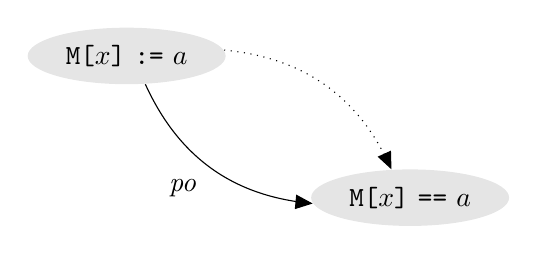
\begin{tikzpicture}
  [scale=.6,auto=left,every node/.style={ellipse,fill=gray!20}]
  \node (n1) at (1,4) {$\texttt{M[}x\texttt{]}~\texttt{:=}~a$};
  \node (n3) at (7,1) {$\texttt{M[}x\texttt{]}~\texttt{==}~a$};

  \draw[dotted,bend left, arrows={-{triangle 45}}] (n1) to (n3);
  \draw[bend right,arrows={-{triangle 45}}] (n1) to (n3);
  \node[fill=none] (x) at (2.63, 1.7) {\rotatebox{-10}{\xmark}};
  \node[fill=none] (po) at (2.2,1.2) {\emph{po}};
\end{tikzpicture}
  \caption{}
  \label{Fig:Intro1}
\end{subfigure}%
\begin{subfigure}{.5\textwidth}
  \centering
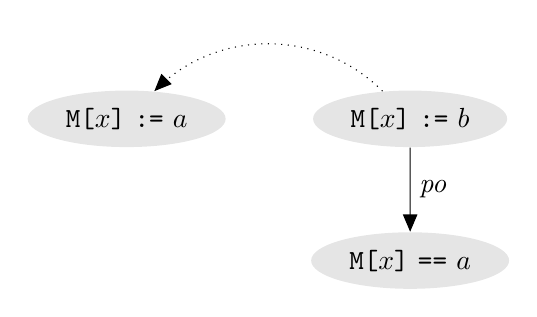
\begin{tikzpicture}
  [scale=.6,auto=left,every node/.style={ellipse,fill=gray!20}]
  \node (n1) at (1,4) {$\texttt{M[}x\texttt{]}~\texttt{:=}~a$};
  \node (n2) at (7,4) {$\texttt{M[}x\texttt{]}~\texttt{:=}~b$};
  \node (n3) at (7,1) {$\texttt{M[}x\texttt{]}~\texttt{==}~a$};

  \draw[arrows={-{triangle 45}}] (n2) to (n3);
  \draw[dotted,arrows={-{triangle 45}}] (n2) to [bend right=45] (n1);
  \node[fill=none] (po) at (7.5,2.5) {\emph{po}};
\end{tikzpicture}
  \caption{}
  \label{Fig:Intro2}
\end{subfigure}%

\caption{Edge-introduction rules. In (a) the dotted memory-order
edge is introduced if the solid program-order edge, labelled
\emph{po}, does not exist.  In (b) the dotted memory-order edge
is introduced if the program-order edge, labelled \emph{po}, exists.}
\label{Fig:IntroRules}
\end{figure}

\begin{figure}[p]
\centering
\begin{subfigure}{.5\textwidth}
  \centering
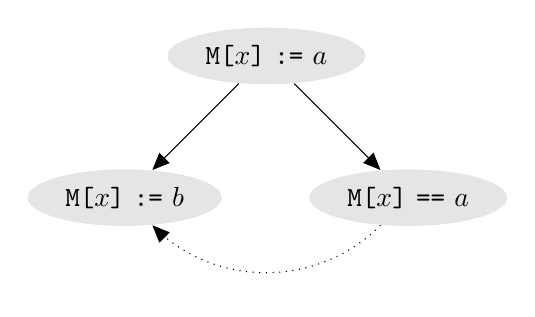
\begin{tikzpicture}
  [scale=.6,auto=left,every node/.style={ellipse,fill=gray!20}]
  \node (n1) at (4,4) {$\texttt{M[}x\texttt{]}~\texttt{:=}~a$};
  \node (n2) at (1,1)  {$\texttt{M[}x\texttt{]}~\texttt{:=}~b$};
  \node (n3) at (7,1)  {$\texttt{M[}x\texttt{]}~\texttt{==}~a$};

  \draw[arrows={-{triangle 45}}] (n1) to (n2);
  \draw[arrows={-{triangle 45}}] (n1) to (n3);
  \draw[dotted,arrows={-{triangle 45}}] (n3) to [bend left=45] (n2);
\end{tikzpicture}
  \caption{}
  \label{Fig:Infer1}
\end{subfigure}%
\begin{subfigure}{.5\textwidth}
  \centering
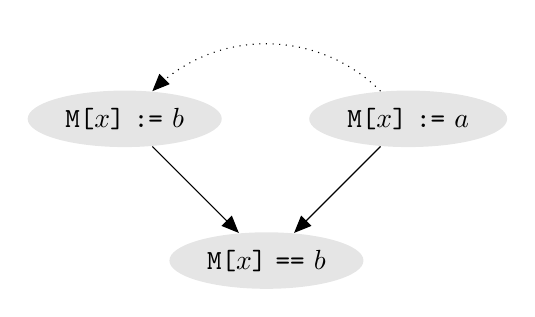
\begin{tikzpicture}
  [scale=.6,auto=left,every node/.style={ellipse,fill=gray!20}]
  \node (n1) at (1,4) {$\texttt{M[}x\texttt{]}~\texttt{:=}~b$};
  \node (n2) at (7,4) {$\texttt{M[}x\texttt{]}~\texttt{:=}~a$};
  \node (n3) at (4,1) {$\texttt{M[}x\texttt{]}~\texttt{==}~b$};

  \draw[arrows={-{triangle 45}}] (n1) to (n3);
  \draw[arrows={-{triangle 45}}] (n2) to (n3);
  \draw[dotted,arrows={-{triangle 45}}] (n2) to [bend right=45] (n1);
\end{tikzpicture}
  \caption{}
  \label{Fig:Infer2}
\end{subfigure}
\caption{Graphical representation of the edge-inference rules proposed by
Manovit\cite{Manovit}.  In
each case, if the solid memory-order edges are known to exist,
either directly or
by transitivity, then the dotted memory-order edge can be inferred.}
\label{Fig:InferRules}
\end{figure}

The key inefficiency of this algorithm is the non-determinism present
in the topological sort.  At any stage, there may exist several store
operations that can be removed next.  If a bad choice is made, the
algorithm must backtrack since an alternative choice may lead to
success.  (The order of stores to each address is not known in
advance.)

\subsubsection*{Reducing non-determinism}

Manovit proposes the two rules shown in Figure \ref{Fig:InferRules} as
a way of inferring new edges in the analysis graph, greatly
reducing the amount of non-determinism in the topological sort.
Notice that applying these rules can introduce edges which enable the
rules to be applied again.  Therefore it is desirable to apply the
rules repeatedly until a fixed-point is reached, i.e. until no new
edges are inferred.

This leads to two modifications of the simple algorithm above: first,
add a new step after step (3) that applies the inference rules until a
fixed-point; second, every time a store is removed from the
graph in step (5), and new edges are added, reapply the inference rules
until a fixed-point.

\subsubsection*{Reducing rule-application sites}

Applying the inference rules at all matching sites in the analysis
graph would be extremely inefficient and, fortunately, unnecessary.
Instead, it is sufficient to apply each rule once for each store $s$
of the form $\texttt{M[}x\texttt{] := } a$ with:

\begin{itemize}

\item for rule \ref{Fig:Infer1}, node $\texttt{M[}x\texttt{] := } b$
bound to the earliest store to address $x$ that non-strictly succeeds
$s$ in the analysis graph;

\item for rule \ref{Fig:Infer2}, node $\texttt{M[}x\texttt{] == } b$
bound to the earliest load to address $x$ that non-strictly succeeds
$s$ in the analysis graph.

\end{itemize}

\noindent While there may exist several bindings that satisfy the
above constraints (the earliest successor may not be unique in a
partial order), the number of application sites to consider is greatly
reduced.

\subsubsection*{Determining the earliest successors}

The problem now is: starting from any store operation, how do we
efficiently determine the next load and store to the same address in
the analysis graph?

To answer this, we maintain two data structures.  The first is the
mapping $nextLoad(op, t, a)$ that gives the next \emph{load} (in the
analysis graph) to address $a$ on thread $t$ from operation $op$.
(Since loads to the same address on a given thread are totally ordered
under all models, this mapping is a function, i.e. unambiguous.)
Initially, it is computed by a backward analysis, propagating the next
load for each $(a, t)$ pair backwards along the edges of the analysis
graph, in reverse-topological order.  At a fork point, the information
at several nodes is merged by taking the minimum program-order load
for each $(a, t)$ pair.  When a new edge $i \rightarrow j$ is added to
the graph, the $nextLoad$ mapping is updated by applying the same
propagation method backwards from node $j$ until no new updates to the
mapping are made.

The second data structure we maintain is the mapping $nextStore$,
identical to $nextLoad$ but giving the next store instead of the next
load.  These two data structures have a number of uses:

\begin{itemize}

\item the inference rules from Figure \ref{Fig:InferRules} can be
applied to the entire analysis graph in linear-time;

\item the existence of a path from a store to any load or store can
be determined in constant-time, avoiding the addition of
redundant edges to the graph;

\item similarly, it can be determined in constant-time whether or not
the addition of an edge to the graph will lead to a cycle, allowing
immediate failure detection;

\item when adding an edge to the graph, the backwards propagation
method used to update the $nextLoad$ and $nextStore$ mappings will
naturally visit the nodes at which the inference rules must be
re-applied.

\end{itemize}

\subsubsection*{Comparison to Manovit's algorithm}

When specialising the algorithm to the TSO model, it is possible to
simplify the $nextLoad$ and $nextStore$ mappings.  Instead of mapping
each $(op, a, t)$ triple to the next load or next store, it is
sufficient to map each $(op, t)$ pair.  This is because all loads by
the same thread are totally ordered under TSO, and so too are all
stores by the same thread.  So for example, once the next load on some
thread is determined, the next load to a particular address on that
thread can be easily found by looking at the static program order.
Consequently, the size of these data structures reduces from $2 \times
N \times A \times T$ for $N$ operations, $A$ addresses, and $T$
threads to $2 \times N \times T$.  Not only does this save space, but
it makes the backwards analysis faster as the amount of information
being propagated is smaller.  In other words, the efficiency of our
checker depends on the number of different address locations used in
the trace.  This is not the case for Manovit's TSO-only checker.


\section{POWER model (POW)}
\label{Section:POWERModel}

The key relaxation introduced by the POW model is to allow writes to
be observed by some threads before they can be observed by others
(known as the ``non-multi-copy-atomic'' property \cite{POWER}).  This
supports two important features found in advanced memory-subsystems:
(1) cache hierarchies involving more than one shared cache; (2) an
optimisation called \emph{lazy invalidation} in which the cache
coherence protocol can buffer invalidate messages (or update
messages) until a \verb!sync! is issued.  Before presenting the model,
we look at a few examples demonstrating this relaxed behaviour.

\paragraph{Example (WRC+deps)}  The following trace is allowed by POW
but forbidden by WMO.

\begin{verbatim}
0: M[0] := 1
1: M[0] == 1    @ 100:110
1: M[1] := 1    @ 115
2: M[1] == 1    @ 200:210
2: M[0] == 0    @ 215
\end{verbatim}

\noindent Notice the dependencies prevent any local reordering of
operations, which is why the trace is forbidden by WMO.  This is an
example of non-multi-copy-atomic behaviour: the write by thread 0
propagates to thread 1 before it propagates to thread 2.  At the
hardware level, this could be explained by the presence of a cache
shared by threads 0 and 1 but not 2, or by a coherence protocol that,
upon seeing the write of thread 0, does not eagerly update the local
cache of thread 2, allowing it to read a stale value.


\paragraph{Example (WRC+sync+dep)} A single \verb'sync' operation,
inserted as follows, is enough to forbid the relaxed behaviour.

\begin{verbatim}
0: M[0] := 1
1: M[0] == 1
1: sync
1: M[1] := 1
2: M[1] == 1    @ 200:210
2: M[0] == 0    @ 215
\end{verbatim}

\noindent This demonstrates the so-called ``cumulative'' property of
\verb!sync! \cite{POWER}: not only does \verb!sync! ensure that all
preceding writes by the issuing thread have propagated to all other
threads, but it also ensures that any writes that the issuing thread
has observed before the \verb!sync! have also propagated.  In this
example, any thread that sees the write by thread 1 must also see the
write by thread 0 because thread 1's write is preceded by a
\verb'sync' which is in turn preceded by an observation of thread 0's
write.

\paragraph{Example (SB+syncs and MP+sync+dep revisited)} Under POW,
these examples are still forbidden: the \verb!sync! instructions are
still are enough to forbid the relaxed behaviour.

\paragraph{Example (WWC+deps)} The following trace is allowed by POW
but forbidden by WMO.

\begin{verbatim}
0: M[0] := 1
1: M[0] == 1 @ 100:110
1: M[1] := 1 @ 115:
2: M[1] == 1 @ 200:210
2: M[0] := 2 @ 215:
final M[0] == 1
\end{verbatim}

\noindent At the hardware level, this example can again be be
explained by the presence of a cache, say $C$, shared by threads 0 and
1 but not 2: (1) the write by thread 0 can reach $C$ and be
observed by thread 1; (2) $C$ can evict the write by thread 1 before
the write by thread 0; (3) thread 2 can observe the write of thread 1
in the last-level cache; (4) the write by thread 2 can reach the
last-level cache; and (5) $C$ can evict the write by thread 0 and
overwrite thread 2's write in the last-level cache.  To our knowledge,
however, this behaviour cannot be explained by the lazy invalidation
optimisation.

\subsection*{Operational Semantics}

Once again, we define the allowed behaviours by way of an abstract
machine with a state and set of state-transition rules.  The state
consists of:

\begin{itemize}

\item A trace $T$ (a sequence of operations in the format given in
\S\ref{Section:TraceFormat}).

\item A \emph{value order} $V(a)$ for each address $a$, represented as
a set of edges between values written to address $a$.

\item A set $W$ of address-value pairs $(a, v)$, representing writes
that have entered the memory-subsystem.

\item A mapping $L$ from a thread-address pair $(t,a)$ to the last
value seen at address $a$ on thread $t$.

\end{itemize}

In the \emph{initial state}, $T$ is the trace we wish to check, $V(a)
= \{\}$ for each address $a$, $W = \{\}$, and $L(t,a) = 0$ for each
thread $t$ and address $a$.

Using the state-transition rules, if there is a path from the initial
state to a state in which $T = []$ and $V(a)$ allows the
\verb#final# constraint on each address $a$, then we say that the
machine accepts the initial trace and that the trace $T$ is allowed by
the model.  Otherwise, it is disallowed by the model.

We first present a machine that ignores atomic read-modify-write
operations, and then extend the machine to support them.

\paragraph{Rule 1}

Non-deterministically pick a thread $t$ and an address $a$.  From the
trace, remove the first operation $i$ on thread $t$ that satisfies the
condition: (a) $i = \texttt{sync}$; or (b) $i$ accesses address $a$
and no operation that precedes $i$ in program-order has an end-time
that precedes the begin-time of $i$.

\begin{enumerate}
\item 
     If $i = \texttt{sync}$ then $\textbf{fail}$.

\item 
     If $i = \texttt{M[}a\texttt{]:=}~v$ then:

\begin{enumerate}
\item
     add $(a, v)$ to set $W$;
\item
     if $L(t,a) \neq v$, add edge $L(t, a) \rightarrow v$ to $V(a)$
     and $\textbf{fail}$ if a cycle is created.
\item
     update $L(t,a)$ to $v$.
\end{enumerate}

\item 
     If $i = \texttt{M[}a\texttt{]==}~v$ then:

\begin{enumerate}
\item
     if $(a, v) \notin W$ then $\textbf{fail}$
\item
     if $L(t,a) \neq v$, add edge $L(t, a) \rightarrow v$ to $V(a)$
     and $\textbf{fail}$ if a cycle is created.
\item
     update $L(t,a)$ to $v$.
\end{enumerate}

\end{enumerate}

\paragraph{Rule 2}

Pick a thread $t$ non-deterministically.  Remove the first operation
$i$ executed by $t$ from the trace.

\begin{enumerate}
\item
     If $i \neq \texttt{sync}$ then $\textbf{fail}$;
\item
     Otherwise, for each address $a$ and thread $t' \neq t$:
\begin{enumerate}
\item
     let $w$ be the next value read from or written to address $a$ by
     thread $t'$ in the trace;
\item
     if $L(t,a) \neq w$ then add edge $L(t,a) \rightarrow w$ to $V(a)$
     and $\textbf{fail}$ if a cycle is created.

\end{enumerate}
\end{enumerate}

\subsection*{Atomic operations}

Atomic read-modify-write operations can be treated simply as adjacent
program-order read and write operations in the above semantics,
provided the following condition is met: for each address $a$ there
must exist a topological sort of $V(a)$ in which $v$ and $w$ are
adjacent for each operation $\texttt{<M[}a\texttt{]==}~v\texttt{;
M[}a\texttt{]:=}~w\texttt{>}$.

\section{Performance}
\label{Section:Performance}

\begin{figure}
\begin{center}
\includegraphics{performance/tso.pdf}
\end{center}
\caption{Performance of TSO checker.}
\label{Graph:TSO}
\end{figure}

\begin{figure}
\begin{center}
\includegraphics{performance/wmo.pdf}
\end{center}
\caption{Performance of WMO checker.}
\label{Graph:WMO}
\end{figure}

\begin{figure}
\begin{center}
\includegraphics{performance/pow.pdf}
\end{center}
\caption{Performance of POW checker with \texttt{-g} flag specified.}
\label{Graph:POW}
\end{figure}



For performance evaluation, we have generated a range of
traces\footnote{Using a model cache implementation with features
including load and store buffering, out-of-order eviction,
out-of-order responses, prefetching and invalidation-based coherence.}
with various numbers of memory operations ($n \in \{8K, 16K, 24K,
32K\})$, threads ($t \in \{4, 16, 32\}$), and addresses ($a \in \{4,
16, 32\}$).  For each combination of parameters, we generate 16
traces, giving 576 traces for each supported model.

Figures \ref{Graph:TSO}, \ref{Graph:WMO}, and \ref{Graph:POW} show how
the performances of the TSO, WMO and POW checkers vary with the number
of operations and threads present, averaged over the number of
addresses present.  In the case of the POW checker, we use the
\verb!-g! flag, specifying a global clock domain and 
enabling the use of begin and end times to infer a partial global
ordering of \verb!sync! operations.  Without the \verb!-g! flag, the
POW checker has a limited completion rate: for 4, 16 and 32 threads
respectively, it has a completion rate of 100\%, 96\%, and 54\%.

\section{Correctness}
\label{Section:Correctness}

\subsection*{Litmus tests}

Axe has been applied to around 200 litmus tests from the PPCMEM
distribution \cite{PPCMEM}, and verified against the outcomes of the
operational models given in \S\ref{Section:SPARCModels} and
\S\ref{Section:POWERModel}, and also against the output of PPCMEM.
The tests are present in the \verb!tests/litmus! subdirectory, and the
outcomes are listed in Appendix A.

\subsection*{Random tests}

Axe has been applied to around 200,000 randomly-generated traces
present in the \verb!tests/random! subdirectory, and verified against
the outcomes of the operational models given in
\S\ref{Section:SPARCModels} and \S\ref{Section:POWERModel}.  Each of
these traces is fairly short, ranging from around 10 to 50 memory
operations in size.

\subsection*{Cache tests}

Axe has been applied to the CHERI cache implementation, and also to
the model cache implementation mentioned in
\S\ref{Section:Performance}, giving the expected outcomes.  For spaces
reasons, we have not included these traces in the Axe
distribution.

\section{Acknowledgements}

Thanks to members of the Semantics group at the University of
Cambridge Computer Laboratory for numerous clarifications about
relaxed memory models.  This work was supported by DARPA/AFRL
contracts FA8750-10-C-0237 (CTSRD) and FA8750-11-C-0249 (MRC2), and
EPSRC grant EP/K008528/1 (REMS).  The views, opinions, and/or findings
contained in this manual are those of the authors and should not be
interpreted as representing the official views or policies, either
expressed or implied, of the Department of Defense or the U.S.
Government.

\begin{thebibliography}{99}
\addcontentsline{toc}{section}{References}
\setlength{\itemsep}{1pt}

\bibitem{BlueCheck} M. Naylor and S. W. Moore, \emph{A generic
synthesisable test bench}, in MEMOCODE 2015, pp. 128--137.

\bibitem{Litmus} J. Alglave, L. Maranget, S. Sarkar, and P.
Sewell, \emph{Litmus: Running Tests Against Hardware}, in TACAS 2011,
pp. 41--44.

\bibitem{SC} L. Lamport.  \emph{How to Make a Multiprocessor Computer
That Correctly Executes Multiprocess Programs}, IEEE Transactions on
Computers, volume 28, number 9, pp. 690--691, 1979.

\bibitem{SPARC} D. L. Weaver and T. Germond. \emph{ The SPARC
Architecture Manual Version 9}, 2003.

\bibitem{POWER} S. Sarkar, P. Sewell, J.  Alglave, L. Maranget, and D.
Williams. \emph{Understanding POWER Multiprocessors}, SIGPLAN Notices,
vol. 46, num. 6, pp. 175--186, June 2011.

\bibitem{CHERI} \emph{Homepage of the CHERI processor (Capability
Hardware Enhanced RISC Instructions)}, \url{http://chericpu.org}.

\bibitem{Gibbons} P. B.  Gibbons and E. Korach.  \emph{On testing
cache-coherent shared memories}, in SPAA 1994, pp.  177–-188.

\bibitem{Manovit} C. Manovit. \emph{Testing memory consistency of
shared-memory multiprocessors}, PhD thesis, Stanford University, 2006.

\bibitem{TSOTool} \emph{Homepage of TSOTool}, a program for verifying
memory systems using the memory consistency model,
\url{http://xenon.stanford.edu/~hangal/tsotool.html}.

\bibitem{ParkDill} S. Park and D. L. Dill.  \emph{ An executable
specification, analyzer and verifier for RMO (relaxed memory order)},
in SPAA 1995.

\bibitem{PPCMEM} \emph{Homepage of PPCMEM/ARMMEM},
a tool for exploring the POWER and ARM memory models,
\url{https://www.cl.cam.ac.uk/~pes20/ppcmem/}.

%\bibitem{Herd} J. Alglave, L. Maranget, M. Tautschnig. \emph{Herding
%Cats: Modelling, Simulation, Testing, and Data Mining for Weak
%Memory}, ACM TOPLAS, vol. 36, num. 2, pp. 7:1--7:74, July 2014.


%\bibitem{MemModels} S. Adve and K. Gharachorloo. \emph{Shared Memory
%Consistency Models: A Tutorial}, Computer Journal, volume 29, number
%12, pp. 66--76, 1996.


\end{thebibliography}

\section*{Appendix A: Litmus test results}
\addcontentsline{toc}{section}{Appendix A: Litmus test results}

The following table gives the output of Axe on a large number of
litmus tests from the PPCMEM distribution.  These tests can also be
found in the Axe distribution in the \verb#tests/litmus# subdirectory.
We use a tick mark (\cmark) to denote that the behaviour described by
the test is allowed, and an empty cell to denote that it is forbidden.
In each case, our POW model gives the same outcome as PPCMEM.  

\begin{longtable}{lccccc}
\textbf{Test name} & \textbf{SC} & \textbf{TSO} &
\textbf{PSO} & \textbf{WMO} & \textbf{POW} \\
\\
\endhead
\texttt{2+2W+sync+po } &  &  & \cmark & \cmark & \cmark \\
\texttt{3.2W } &  &  & \cmark & \cmark & \cmark \\
\texttt{3.2W+sync+po+po } &  &  & \cmark & \cmark & \cmark \\
\texttt{3.2W+syncs } &  &  &  &  &  \\
\texttt{3.2W+sync+sync+po } &  &  & \cmark & \cmark & \cmark \\
\texttt{3.LB+addr+addr+po } &  &  &  & \cmark & \cmark \\
\texttt{3.LB+addr+po+po } &  &  &  & \cmark & \cmark \\
\texttt{3.LB+addrs } &  &  &  &  &  \\
\texttt{3.LB+addr+sync+po } &  &  &  & \cmark & \cmark \\
\texttt{3.LB } &  &  &  & \cmark & \cmark \\
\texttt{3.LB+sync+addr+addr } &  &  &  &  &  \\
\texttt{3.LB+sync+addr+po } &  &  &  & \cmark & \cmark \\
\texttt{3.LB+sync+po+po } &  &  &  & \cmark & \cmark \\
\texttt{3.LB+syncs } &  &  &  &  &  \\
\texttt{3.LB+sync+sync+addr } &  &  &  &  &  \\
\texttt{3.LB+sync+sync+po } &  &  &  & \cmark & \cmark \\
\texttt{3.SB } &  & \cmark & \cmark & \cmark & \cmark \\
\texttt{3.SB+sync+po+po } &  & \cmark & \cmark & \cmark & \cmark \\
\texttt{3.SB+syncs } &  &  &  &  &  \\
\texttt{3.SB+sync+sync+po } &  & \cmark & \cmark & \cmark & \cmark \\
\texttt{IRIW+addr+po } &  &  &  & \cmark & \cmark \\
\texttt{IRIW+addrs } &  &  &  &  & \cmark \\
\texttt{IRIW } &  &  &  & \cmark & \cmark \\
\texttt{IRIW+sync+addr } &  &  &  &  & \cmark \\
\texttt{IRIW+sync+po } &  &  &  & \cmark & \cmark \\
\texttt{IRIW+syncs } &  &  &  &  &  \\
\texttt{IRRWIW+addr+po } &  &  &  & \cmark & \cmark \\
\texttt{IRRWIW+addrs } &  &  &  &  & \cmark \\
\texttt{IRRWIW+addr+sync } &  &  &  &  & \cmark \\
\texttt{IRRWIW } &  &  &  & \cmark & \cmark \\
\texttt{IRRWIW+po+addr } &  &  &  & \cmark & \cmark \\
\texttt{IRRWIW+po+sync } &  &  &  & \cmark & \cmark \\
\texttt{IRRWIW+sync+addr } &  &  &  &  & \cmark \\
\texttt{IRRWIW+sync+po } &  &  &  & \cmark & \cmark \\
\texttt{IRRWIW+syncs } &  &  &  &  &  \\
\texttt{IRWIW+addr+po } &  &  &  & \cmark & \cmark \\
\texttt{IRWIW+addrs } &  &  &  &  & \cmark \\
\texttt{IRWIW } &  &  &  & \cmark & \cmark \\
\texttt{IRWIW+sync+addr } &  &  &  &  & \cmark \\
\texttt{IRWIW+sync+po } &  &  &  & \cmark & \cmark \\
\texttt{IRWIW+syncs } &  &  &  &  &  \\
\texttt{ISA2+sync+addr+addr } &  &  &  &  &  \\
\texttt{ISA2+sync+addr+po } &  &  &  & \cmark & \cmark \\
\texttt{ISA2+sync+addr+sync } &  &  &  &  &  \\
\texttt{ISA2+sync+po+addr } &  &  &  & \cmark & \cmark \\
\texttt{ISA2+sync+po+po } &  &  &  & \cmark & \cmark \\
\texttt{ISA2+sync+po+sync } &  &  &  & \cmark & \cmark \\
\texttt{ISA2+syncs } &  &  &  &  &  \\
\texttt{ISA2+sync+sync+addr } &  &  &  &  &  \\
\texttt{ISA2+sync+sync+po } &  &  &  & \cmark & \cmark \\
\texttt{LB+addr+po } &  &  &  & \cmark & \cmark \\
\texttt{LB+addrs } &  &  &  &  &  \\
\texttt{LB } &  &  &  & \cmark & \cmark \\
\texttt{LB+sync+addr } &  &  &  &  &  \\
\texttt{LB+sync+po } &  &  &  & \cmark & \cmark \\
\texttt{LB+syncs } &  &  &  &  &  \\
\texttt{MP } &  &  & \cmark & \cmark & \cmark \\
\texttt{MP+po+addr } &  &  & \cmark & \cmark & \cmark \\
\texttt{MP+po+sync } &  &  & \cmark & \cmark & \cmark \\
\texttt{MP+sync+addr } &  &  &  &  &  \\
\texttt{MP+sync+po } &  &  &  & \cmark & \cmark \\
\texttt{MP+syncs } &  &  &  &  &  \\
\texttt{R } &  & \cmark & \cmark & \cmark & \cmark \\
\texttt{R+po+sync } &  &  & \cmark & \cmark & \cmark \\
\texttt{R+sync+po } &  & \cmark & \cmark & \cmark & \cmark \\
\texttt{R+syncs } &  &  &  &  &  \\
\texttt{RWC+addr+po } &  & \cmark & \cmark & \cmark & \cmark \\
\texttt{RWC+addr+sync } &  &  &  &  & \cmark \\
\texttt{RWC } &  & \cmark & \cmark & \cmark & \cmark \\
\texttt{RWC+po+sync } &  &  &  & \cmark & \cmark \\
\texttt{RWC+sync+po } &  & \cmark & \cmark & \cmark & \cmark \\
\texttt{RWC+syncs } &  &  &  &  &  \\
\texttt{S } &  &  & \cmark & \cmark & \cmark \\
\texttt{SB } &  & \cmark & \cmark & \cmark & \cmark \\
\texttt{SB+sync+po } &  & \cmark & \cmark & \cmark & \cmark \\
\texttt{SB+syncs } &  &  &  &  &  \\
\texttt{S+po+addr } &  &  & \cmark & \cmark & \cmark \\
\texttt{S+po+sync } &  &  & \cmark & \cmark & \cmark \\
\texttt{S+sync+addr } &  &  &  &  &  \\
\texttt{S+sync+po } &  &  &  & \cmark & \cmark \\
\texttt{S+syncs } &  &  &  &  &  \\
\texttt{WRC+addr+po } &  &  &  & \cmark & \cmark \\
\texttt{WRC+addrs } &  &  &  &  & \cmark \\
\texttt{WRC+addr+sync } &  &  &  &  & \cmark \\
\texttt{WRC } &  &  &  & \cmark & \cmark \\
\texttt{WRC+po+addr } &  &  &  & \cmark & \cmark \\
\texttt{WRC+po+sync } &  &  &  & \cmark & \cmark \\
\texttt{WRC+sync+addr } &  &  &  &  &  \\
\texttt{WRC+sync+po } &  &  &  & \cmark & \cmark \\
\texttt{WRC+syncs } &  &  &  &  &  \\
\texttt{WRR+2W+addr+po } &  &  & \cmark & \cmark & \cmark \\
\texttt{WRR+2W+addr+sync } &  &  &  &  & \cmark \\
\texttt{WRR+2W } &  &  & \cmark & \cmark & \cmark \\
\texttt{WRR+2W+po+sync } &  &  &  & \cmark & \cmark \\
\texttt{WRR+2W+sync+po } &  &  & \cmark & \cmark & \cmark \\
\texttt{WRR+2W+syncs } &  &  &  &  &  \\
\texttt{WRW+2W+addr+po } &  &  & \cmark & \cmark & \cmark \\
\texttt{WRW+2W+addr+sync } &  &  &  &  & \cmark \\
\texttt{WRW+2W } &  &  & \cmark & \cmark & \cmark \\
\texttt{WRW+2W+po+sync } &  &  &  & \cmark & \cmark \\
\texttt{WRW+2W+sync+po } &  &  & \cmark & \cmark & \cmark \\
\texttt{WRW+2W+syncs } &  &  &  &  &  \\
\texttt{W+RWC } &  & \cmark & \cmark & \cmark & \cmark \\
\texttt{W+RWC+po+addr+po } &  & \cmark & \cmark & \cmark & \cmark \\
\texttt{W+RWC+po+addr+sync } &  &  & \cmark & \cmark & \cmark \\
\texttt{W+RWC+po+po+sync } &  &  & \cmark & \cmark & \cmark \\
\texttt{W+RWC+po+sync+po } &  & \cmark & \cmark & \cmark & \cmark \\
\texttt{W+RWC+po+sync+sync } &  &  & \cmark & \cmark & \cmark \\
\texttt{W+RWC+sync+addr+po } &  & \cmark & \cmark & \cmark & \cmark \\
\texttt{W+RWC+sync+addr+sync } &  &  &  &  &  \\
\texttt{W+RWC+sync+po+po } &  & \cmark & \cmark & \cmark & \cmark \\
\texttt{W+RWC+sync+po+sync } &  &  &  & \cmark & \cmark \\
\texttt{W+RWC+syncs } &  &  &  &  &  \\
\texttt{W+RWC+sync+sync+po } &  & \cmark & \cmark & \cmark & \cmark \\
\texttt{WRW+WR+addr+po } &  & \cmark & \cmark & \cmark & \cmark \\
\texttt{WRW+WR+addr+sync } &  &  &  &  & \cmark \\
\texttt{WRW+WR } &  & \cmark & \cmark & \cmark & \cmark \\
\texttt{WRW+WR+po+sync } &  &  &  & \cmark & \cmark \\
\texttt{WRW+WR+sync+po } &  & \cmark & \cmark & \cmark & \cmark \\
\texttt{WRW+WR+syncs } &  &  &  &  &  \\
\texttt{WWC+addr+po } &  &  &  & \cmark & \cmark \\
\texttt{WWC+addrs } &  &  &  &  & \cmark \\
\texttt{WWC+addr+sync } &  &  &  &  & \cmark \\
\texttt{WWC } &  &  &  & \cmark & \cmark \\
\texttt{WWC+po+addr } &  &  &  & \cmark & \cmark \\
\texttt{WWC+po+sync } &  &  &  & \cmark & \cmark \\
\texttt{WWC+sync+addr } &  &  &  &  &  \\
\texttt{WWC+sync+po } &  &  &  & \cmark & \cmark \\
\texttt{WWC+syncs } &  &  &  &  &  \\
\texttt{Z6.0 } &  & \cmark & \cmark & \cmark & \cmark \\
\texttt{Z6.0+po+addr+po } &  & \cmark & \cmark & \cmark & \cmark \\
\texttt{Z6.0+po+addr+sync } &  &  & \cmark & \cmark & \cmark \\
\texttt{Z6.0+po+po+sync } &  &  & \cmark & \cmark & \cmark \\
\texttt{Z6.0+po+sync+po } &  & \cmark & \cmark & \cmark & \cmark \\
\texttt{Z6.0+po+sync+sync } &  &  & \cmark & \cmark & \cmark \\
\texttt{Z6.0+sync+addr+po } &  & \cmark & \cmark & \cmark & \cmark \\
\texttt{Z6.0+sync+addr+sync } &  &  &  &  &  \\
\texttt{Z6.0+sync+po+po } &  & \cmark & \cmark & \cmark & \cmark \\
\texttt{Z6.0+sync+po+sync } &  &  &  & \cmark & \cmark \\
\texttt{Z6.0+syncs } &  &  &  &  &  \\
\texttt{Z6.0+sync+sync+po } &  & \cmark & \cmark & \cmark & \cmark \\
\texttt{Z6.1 } &  &  & \cmark & \cmark & \cmark \\
\texttt{Z6.1+po+po+addr } &  &  & \cmark & \cmark & \cmark \\
\texttt{Z6.1+po+po+sync } &  &  & \cmark & \cmark & \cmark \\
\texttt{Z6.1+po+sync+addr } &  &  & \cmark & \cmark & \cmark \\
\texttt{Z6.1+po+sync+po } &  &  & \cmark & \cmark & \cmark \\
\texttt{Z6.1+po+sync+sync } &  &  & \cmark & \cmark & \cmark \\
\texttt{Z6.1+sync+po+addr } &  &  & \cmark & \cmark & \cmark \\
\texttt{Z6.1+sync+po+po } &  &  & \cmark & \cmark & \cmark \\
\texttt{Z6.1+sync+po+sync } &  &  & \cmark & \cmark & \cmark \\
\texttt{Z6.1+syncs } &  &  &  &  &  \\
\texttt{Z6.1+sync+sync+addr } &  &  &  &  &  \\
\texttt{Z6.1+sync+sync+po } &  &  &  & \cmark & \cmark \\
\texttt{Z6.2 } &  &  & \cmark & \cmark & \cmark \\
\texttt{Z6.2+po+addr+addr } &  &  & \cmark & \cmark & \cmark \\
\texttt{Z6.2+po+addr+po } &  &  & \cmark & \cmark & \cmark \\
\texttt{Z6.2+po+addr+sync } &  &  & \cmark & \cmark & \cmark \\
\texttt{Z6.2+po+po+addr } &  &  & \cmark & \cmark & \cmark \\
\texttt{Z6.2+po+po+sync } &  &  & \cmark & \cmark & \cmark \\
\texttt{Z6.2+po+sync+addr } &  &  & \cmark & \cmark & \cmark \\
\texttt{Z6.2+po+sync+po } &  &  & \cmark & \cmark & \cmark \\
\texttt{Z6.2+po+sync+sync } &  &  & \cmark & \cmark & \cmark \\
\texttt{Z6.2+sync+addr+addr } &  &  &  &  &  \\
\texttt{Z6.2+sync+addr+po } &  &  &  & \cmark & \cmark \\
\texttt{Z6.2+sync+addr+sync } &  &  &  &  &  \\
\texttt{Z6.2+sync+po+addr } &  &  &  & \cmark & \cmark \\
\texttt{Z6.2+sync+po+po } &  &  &  & \cmark & \cmark \\
\texttt{Z6.2+sync+po+sync } &  &  &  & \cmark & \cmark \\
\texttt{Z6.2+syncs } &  &  &  &  &  \\
\texttt{Z6.2+sync+sync+addr } &  &  &  &  &  \\
\texttt{Z6.2+sync+sync+po } &  &  &  & \cmark & \cmark \\
\texttt{Z6.3 } &  &  & \cmark & \cmark & \cmark \\
\texttt{Z6.3+po+po+addr } &  &  & \cmark & \cmark & \cmark \\
\texttt{Z6.3+po+po+sync } &  &  & \cmark & \cmark & \cmark \\
\texttt{Z6.3+po+sync+addr } &  &  & \cmark & \cmark & \cmark \\
\texttt{Z6.3+po+sync+po } &  &  & \cmark & \cmark & \cmark \\
\texttt{Z6.3+po+sync+sync } &  &  & \cmark & \cmark & \cmark \\
\texttt{Z6.3+sync+po+addr } &  &  & \cmark & \cmark & \cmark \\
\texttt{Z6.3+sync+po+po } &  &  & \cmark & \cmark & \cmark \\
\texttt{Z6.3+sync+po+sync } &  &  & \cmark & \cmark & \cmark \\
\texttt{Z6.3+syncs } &  &  &  &  &  \\
\texttt{Z6.3+sync+sync+addr } &  &  &  &  &  \\
\texttt{Z6.3+sync+sync+po } &  &  &  & \cmark & \cmark \\
\texttt{Z6.4 } &  & \cmark & \cmark & \cmark & \cmark \\
\texttt{Z6.4+po+po+sync } &  & \cmark & \cmark & \cmark & \cmark \\
\texttt{Z6.4+po+sync+po } &  & \cmark & \cmark & \cmark & \cmark \\
\texttt{Z6.4+po+sync+sync } &  &  & \cmark & \cmark & \cmark \\
\texttt{Z6.4+sync+po+po } &  & \cmark & \cmark & \cmark & \cmark \\
\texttt{Z6.4+sync+po+sync } &  & \cmark & \cmark & \cmark & \cmark \\
\texttt{Z6.4+syncs } &  &  &  &  &  \\
\texttt{Z6.4+sync+sync+po } &  & \cmark & \cmark & \cmark & \cmark \\
\texttt{Z6.5 } &  & \cmark & \cmark & \cmark & \cmark \\
\texttt{Z6.5+po+po+sync } &  &  & \cmark & \cmark & \cmark \\
\texttt{Z6.5+po+sync+po } &  & \cmark & \cmark & \cmark & \cmark \\
\texttt{Z6.5+po+sync+sync } &  &  & \cmark & \cmark & \cmark \\
\texttt{Z6.5+sync+po+po } &  & \cmark & \cmark & \cmark & \cmark \\
\texttt{Z6.5+sync+po+sync } &  &  & \cmark & \cmark & \cmark \\
\texttt{Z6.5+syncs } &  &  &  &  &  \\
\texttt{Z6.5+sync+sync+po } &  & \cmark & \cmark & \cmark & \cmark \\
\\
Count & 0 & 35 & 89 & 140 & 155
\end{longtable}



\end{document}
